\documentclass{article}
\usepackage{tikz}
\usepackage[nowarning]{braids}
\usetikzlibrary{braids}
\begin{document}
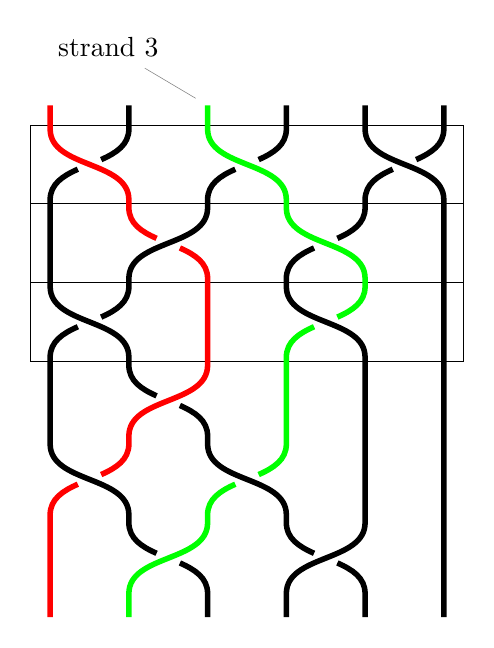
\begin{tikzpicture}
\braid[
  style all floors={fill=yellow},
  line width=2pt,
  style strands={1}{red},
  style strands={3}{green}
] (strands) at (2,0) | s_1-s_3-s_5 | s_2^{-1}-s_4| s_1-s_4 s_2^{-1} s_1-s_3 s_2^{-1}-s_4^{-1};
\typeout{PROBE3s:\expandafter\meaning\csname pgf@sh@ns@strands-3-s\endcsname}
\node[at=(strands-3-s),pin=north west:strand 3] {};
\end{tikzpicture}
\end{document}
